% !TeX program = xelatex
% !TeX encoding = UTF-8
\documentclass{MathorCupmodeling}
\let\kaishu\relax
\newCJKfontfamily\kaishu{KaiTi}[AutoFakeBold] %use fake KaiTi
\usepackage{zhlipsum,mwe}%use random characters
\usepackage{mathtools}%use mathtools
\usepackage{amsmath}
\usepackage{siunitx}
\usepackage{graphicx}
\usepackage{enumitem}
\setlist{nosep}

\begin{document}
\begin{center}
{\Large 开题}

\end{center}
    \newpage

%-------------------------------------------------------------------

	\section{概述}

\subsection{直线一级倒立摆系统介绍}

倒立摆系统是一个非线性自然不稳定系统,是进行控制理论教学及开展各种控制实验的理想实验平台。许多抽象的控制概念如控制系统的稳定性、可控性、系统收敛速度和系统抗干扰能力等,都可以通过倒立摆系统直观的表现出来。对其基础的理论控制以及算法的学习都有十分巨大的帮助。由于倒立摆本身所具有的高阶次,不稳定,多变量。非线性,和强耦合性,许多现代控制理论的研究人员一直将它作为典型的研究对象,不断从中发掘新的控制策略和控制算法,相关的科研成果在航天科技和机器人学方面获得广阔的应用。

本次所用的倒立摆为固高科技公司的直线一级摆:直线倒立摆在直线运动模块(小车)上装有摆杆和角度编码器,直线运动模块有一个自由度,在伺服电机的驱动下可以沿导轨水平运动。

\begin{figure}[hbpt]
\centering
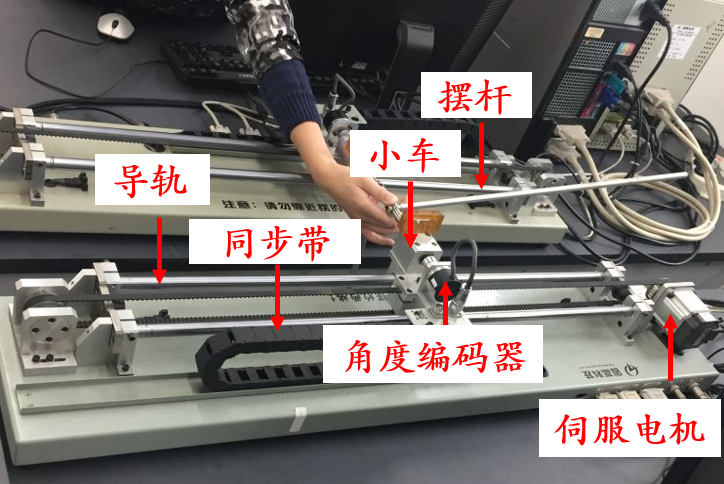
\includegraphics[width=12cm]{实物.png}
\caption{倒立摆系统}\label{实物}
\end{figure}


\subsection{前期准备}

倒立摆系统的控制,可以采用经典的$PID$控制方法,$LQR$控制,模糊控制法,神经网络控制算法,根轨迹控制算法等,我们组搜集了$LQR$,模糊算法,神经网络算法,以及$PID$相关方面的资料,进行比较整理,从四种方法中选取了$LQR$和模糊控制算法进行研究设计。并对研究内容,进度规划,报告,答辩进行了细致的分工,按照计划甘特图推进课程设计。

\subsection{资料准备}


根据查找的文献资料,我们简单总结了四种控制方法的优缺点,现罗列如下

\subsubsection{$LQR$(线性二次型调节器)}
\begin{enumerate}
\item 较好的控制住摆杆并且响应速度较快,超调量。
\item 可以使目标函数达到最优,可以对能控系统进行任意的极点配置来满足所设计系统的性能要求,提高闭环系统的相对稳定性或者使不稳定系统得以镇定。
\item 具有较强的鲁棒性。
\item 对小车的控制效果稍差。
\item $LQR$需要调整两个矩阵,要求解$Riccati$方程确定$Q$和$R$权矩阵,算法复杂。
\end{enumerate}

\subsubsection{神经网络}
\begin{enumerate}
\item 非线性映射,能以任意精度逼近任何非线性连续函数,适合求解内部机制复杂问题。
\item 输入输出变量数目是任意的。
\item 具有自学习和自适应的能力,能过学习获取输出数据间的对应关系,将学习内容存储到网络权值中,具有容错能力,部分神经元受损对全局训练结果不会有很大影响。
\item 存在实时性和自适应性相互矛盾的问题,不能保证快速性和有效性。
\item 权值容易收敛到局部最小点,收敛速度慢,隐含层数目难以确定,训练依赖样本数据,样本数据有采集难度。
\end{enumerate}

\subsubsection{模糊控制}
\begin{enumerate}
\item 使用语言方法,可不需要过程的精确数学模型;
\item 鲁棒性强,适于解决过程控制中的非线性、强耦合时变、滞后等问题;
\item 有较强的容错能力。具有适应受控对象动力学特征变化、环境特征变化和动行条件变化的能力;
\item 模糊控制的设计尚缺乏系统性,这对复杂系统的控制是难以奏效的。难以建立一套系统的模糊控制理论,以解决模糊控制的机理、稳定性分析、系统化设计方法等一系列问题;
\item 如何获得模糊规则及隶属函数即系统的设计办法,完全凭经验进行;
\item 信息简单的模糊处理将导致系统的控制精度降低和动态品质变差。若要提高精度就必然增加量化级数,导致规则搜索范围扩大,降低决策速度,甚至不能进行实时控制;
\end{enumerate}

\subsubsection{$PID$控制}
\begin{enumerate}
\item 原理结构简单,易于实现,使用方便,PID各参数相互独立,可以根据过程的动态特性及时调节。
\item 适用性强,可通过适当简化将非线性的、时变的被控对象变成基本线性和动态特性不随时间变化的系统,应用范围十分广泛,理论成熟。
\item 棒性较好,即其控制品质对被控对象特性的变化不太敏感。
\item 稳定性差,在控制非线性、时变、耦合及参数和结构不确定的复杂过程时,效果不好。
\end{enumerate}

\subsection{题目数据}

将题目的数据整理如\cref{参数}

\begin{table}[h]
\centering
\begin{tabular}{ccc}
\hline
参数 & 意义           & 数值                            \\ \hline
$M$  & 小车质量         & $1.096kg$                       \\ \hline
$m$ & 摆杆质量         & $0.109kg$                       \\ \hline
$l$  & 摆杆质心到转动轴心的长度 & $0.25m$                         \\ \hline
$b$  & 摩擦比例系数       & $0.1N.s/m$                      \\ \hline
$I$  & 摆杆对质心的转动惯量   & $0.0034kg.m^2$ \\ \hline
$T$  & 采样时间         & $0.005s$                        \\ \hline
\end{tabular}
\caption{题目参数}\label{参数}
\end{table}

%-------------------------------------------------------------------
\end{document}